\section{Gas Measurement and Optimization}
\label{sec:gas}

\subsection{Method}
\paragraph{Fair baseline.} Member B left the contracts untouched in Stage 2, so the baseline was
measured first thing in Stage 3, on the contracts exactly as handed over (tag \code{handoff\_2} plus
Member B's B-1 fix), and committed before any contract change (commit \code{2c63365}).

\paragraph{Scenario.} \code{scripts/measureGas.js} plays one complete circle and records the gas of
every state changing call: 4 members, 1,000 mUSD per round, 30 day rounds; everyone pays round 1, then
the round 1 recipient stops paying for rounds 2 to 4 and the circle completes. It also records the
one off deployment cost of each contract, the bytecode sizes, and the sum over every transaction of
the circle (\enquote{whole circle}). The payout order is random, so every action is chosen by payout
\emph{position}, not by account; the numbers are therefore identical on every run (checked by
running the script twice). The Hardhat gas reporter over the full test suite is kept as a second
source (\code{docs/gas/reporter\_baseline.txt}, \code{reporter\_final.txt}).

\paragraph{Cost model.} Since the Berlin and London upgrades \cite{eip2929,eip3529}, the first read of a
storage slot in a transaction costs 2,100 gas and later reads 100; writing a zero slot to a non zero
value costs 20,000 (plus 2,100 if cold) and changing a non zero value 2,900. Calling another
contract costs 2,600 the first time. The optimizations therefore aim at fewer storage slots, fewer
first time writes and fewer external calls.

\paragraph{Procedure.} One optimization per commit, the full test suite after each, and a measurement
after each, so the effect of every optimization is isolated (\code{docs/gas/steps/}). The final
column also contains the three security fixes of Section~\ref{sec:security}.

\subsection{Results}
Table~\ref{tab:gas} is generated from the recorded measurements by a script
(\code{gasSheet.js}); the same table is kept in the repository as the gas sheet. Columns are
cumulative: each adds one optimization to the previous one.

\begin{table}[H]
\centering\footnotesize
\setlength{\tabcolsep}{3.4pt}
\caption{Gas per call, baseline and after each optimization}
\label{tab:gas}
\begin{tabular}{@{}lrrrrrrr@{}}
\toprule
Operation & Baseline & +G1 & +G2 & +G3 & +G4 & Final & Change \\
 & & clones & packing & bitmap & events & (+S1--S3) & \\
\midrule
W1 createCircle & 4,024,450 & 691,217 & 467,767 & 467,767 & 467,767 & 489,638 & $-$87.8\% \\
W2 join (first) & 302,600 & 325,163 & 312,783 & 312,783 & 245,815 & 245,797 & $-$18.8\% \\
W2 join (middle) & 251,300 & 253,963 & 241,583 & 241,583 & 174,615 & 174,597 & $-$30.5\% \\
W2 join (last, starts draw) & 563,251 & 565,914 & 488,542 & 488,542 & 421,574 & 423,556 & $-$24.8\% \\
W3 commit & 75,281 & 75,281 & 54,462 & 54,462 & 54,462 & 54,462 & $-$27.7\% \\
W3 reveal (first) & 104,584 & 104,584 & 62,459 & 62,459 & 62,459 & 62,712 & $-$40.0\% \\
W3 reveal (last) & 70,384 & 70,384 & 45,359 & 45,359 & 45,359 & 45,612 & $-$35.2\% \\
W3 finalizeDraw & 437,077 & 439,740 & 400,892 & 400,892 & 400,892 & 382,944 & $-$12.4\% \\
W4 contribute (first in round) & 129,698 & 132,361 & 124,153 & 103,933 & 103,933 & 102,332 & $-$21.1\% \\
W4 contribute (later) & 95,498 & 98,161 & 89,953 & 69,733 & 69,733 & 68,132 & $-$28.7\% \\
W5 settleRound (all paid) & 173,029 & 175,692 & 103,966 & 104,065 & 104,065 & 102,962 & $-$40.5\% \\
W5 settleRound (one default) & 315,055 & 317,718 & 224,542 & 212,875 & 163,007 & 162,286 & $-$48.5\% \\
W6 claimPayout & 41,586 & 43,716 & 42,032 & 42,032 & 42,032 & 42,032 & +1.1\% \\
W5+W7 last settle (completes) & 539,886 & 542,549 & 434,234 & 424,567 & 225,095 & 223,494 & $-$58.6\% \\
\midrule
\textbf{Whole circle} & \textbf{9,619,893} & 6,373,666 & 5,402,047 & 5,106,285 & 4,539,205 & \textbf{4,521,109} & \textbf{$-$53.0\%} \\
\bottomrule
\end{tabular}
\end{table}

\begin{figure}[H]
\centering
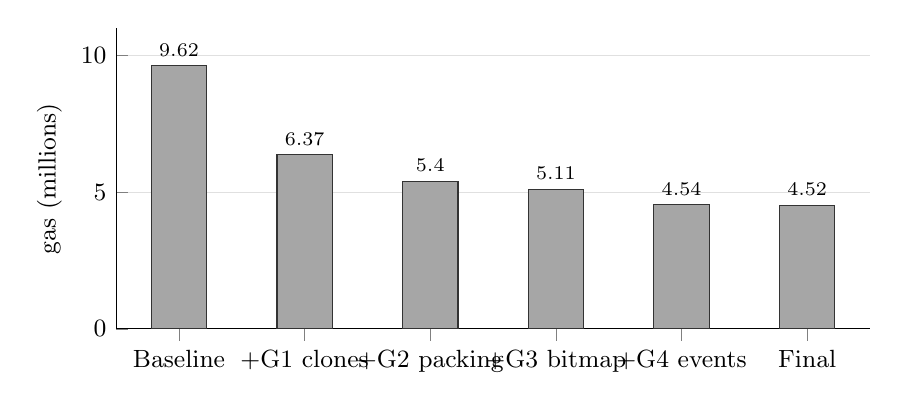
\begin{tikzpicture}
\begin{axis}[
  width=0.92\textwidth, height=5.4cm,
  ybar, bar width=20pt,
  ymin=0, ymax=11,
  ylabel={gas (millions)}, ylabel style={font=\small},
  xtick={1,...,6}, xticklabels={Baseline, +G1 clones, +G2 packing, +G3 bitmap, +G4 events, Final},
  xticklabel style={font=\small},
  yticklabel style={font=\small},
  nodes near coords, nodes near coords style={font=\scriptsize},
  every node near coord/.append style={/pgf/number format/.cd, fixed, precision=2},
  axis lines*=left, ymajorgrids, grid style={black!12},
  enlarge x limits=0.1]
\addplot[fill=black!35, draw=black!80] coordinates {
  (1,9.62) (2,6.37) (3,5.40) (4,5.11) (5,4.54) (6,4.52)};
\end{axis}
\end{tikzpicture}
\caption{Gas for a whole 4 member circle with one default (every transaction), after each step}
\label{fig:gastotal}
\end{figure}

\begin{figure}[H]
\centering
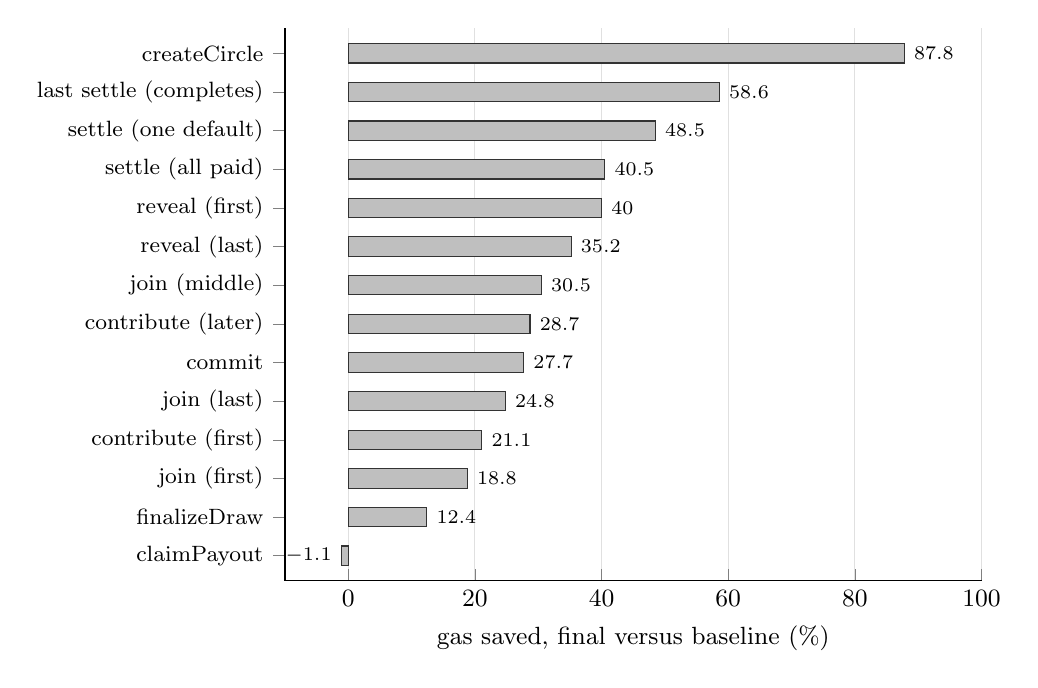
\begin{tikzpicture}
\begin{axis}[
  width=0.86\textwidth, height=8.6cm,
  xbar, bar width=7pt,
  xmin=-10, xmax=100,
  xlabel={gas saved, final versus baseline (\%)}, xlabel style={font=\small},
  ytick={1,...,14},
  yticklabels={claimPayout, finalizeDraw, join (first), contribute (first), join (last), commit, contribute (later), join (middle), reveal (last), reveal (first), settle (all paid), settle (one default), last settle (completes), createCircle},
  yticklabel style={font=\footnotesize},
  xticklabel style={font=\small},
  nodes near coords, nodes near coords style={font=\scriptsize},
  every node near coord/.append style={/pgf/number format/.cd, fixed, precision=1},
  axis lines*=left, xmajorgrids, grid style={black!12},
  enlarge y limits=0.05]
\addplot[fill=black!25, draw=black!80] coordinates {
  (-1.1,1) (12.4,2) (18.8,3) (21.1,4) (24.8,5) (27.7,6) (28.7,7) (30.5,8) (35.2,9) (40.0,10) (40.5,11) (48.5,12) (58.6,13) (87.8,14)};
\end{axis}
\end{tikzpicture}
\caption{Gas saved per operation (negative: the clone's delegatecall makes \code{claimPayout} 446 gas dearer)}
\label{fig:gaspct}
\end{figure}

\subsection{G1: EIP 1167 minimal proxy clones}
The baseline factory deployed a full 16.5 KB \code{Circle} for every committee. Now the factory deploys
one implementation in its constructor and every \code{createCircle} creates a 45 byte clone that
delegates every call to it \cite{eip1167}. \code{Circle} was already set up by \code{initialize} instead of
a constructor (clones never run constructors), and its \code{factory} address is an immutable, so it is
part of the implementation's code and is the same for every clone.

\begin{lstlisting}[language=Solidity]
constructor(...) {
    ...
    implementation = address(new Circle(token_, vault_, payoutOrder_, reputation_));
}
function createCircle(Circle.Config calldata cfg) external returns (address circle) {
    Circle c = Circle(Clones.clone(implementation));   // 45 bytes of code
    c.initialize(cfg, Circle.Modules({...}), msg.sender, admin); // same transaction
    ...
}
\end{lstlisting}

\emph{Effect:} \code{createCircle} from 4,024,450 to 691,217 gas ($-$82.8\%) on its own.
\emph{Cost:} every call into a circle pays about 2,700 gas more for the delegatecall, and a clone's
reentrancy guard slot starts at zero, so the first guarded call (the first join) pays about 20,000
gas once instead of the constructor paying it. Deployment is 780,983 gas dearer because the factory
deploys the implementation, which the first circle repays 4.5 times over.

\subsection{G2: storage packing and immutables}
Every value was a full 32 byte slot in the baseline. Now values that are always small share slots,
sized for their real range (timestamps in 40 bits, durations in 32, the contribution in 64, counts in 8
or 16) following the compiler's packing rules \cite{soliditylayout}, and \code{initialize} \emph{rejects} any value that would not fit instead of truncating it
(attack test A9). The four module addresses are the same for every clone of a factory, so they became
immutables of the implementation and cost no storage at all. To keep the interface, every baseline
public getter (\code{config()}, \code{rounds(r)}, \code{positionOf}, \code{hasPaid}, \dots) is now a view
function with exactly the same outputs.

\begin{table}[H]
\centering\small
\caption{Storage slots used, baseline and final}
\label{tab:slots}
\begin{tabularx}{\textwidth}{@{}LRR@{}}
\toprule
Data & Baseline & Final \\
\midrule
\code{Circle}: configuration, timing, round counter, state, pause fields, module addresses & 17 slots & 3 slots \\
\code{Circle}: per member (position, removed flag, defaults) & 3 slots & 1 slot \\
\code{Circle}: per round (who paid, paid count, result) & $n$ + 5 slots & 2 slots (+1 if short) \\
\code{PayoutOrder}: per draw (flags, deadlines, counters, seed, members) & 7 slots & 3 slots \\
\code{PayoutOrder}: per member (participant, revealed) & 2 slots & 1 slot \\
\code{ReputationRegistry}: per address (record and history) & 3 + 2 per entry & 1 slot \\
\bottomrule
\end{tabularx}
\end{table}

\begin{table}[H]
\centering\small
\caption{Final layout of \code{Circle}'s packed slots (\code{npm run storage:layout})}
\label{tab:layout}
\begin{tabularx}{\textwidth}{@{}P{1cm}LP{1.6cm}@{}}
\toprule
Slot & Fields (bytes) & Used \\
\midrule
3 & \code{state} (1), \code{\_pauseExpiresAt} (5), \code{\_pausedAt} (5), \code{\_pausedTotal} (5), \code{\_lastPauseEnd} (5), \code{\_contribution} (8), \code{\_groupSize} (1), \code{\_maxDefaults} (2) & 32 of 32 \\
4 & \code{organizer} (20), \code{\_joinDuration} (4), \code{\_drawPhaseDuration} (4) & 28 of 32 \\
5 & \code{\_joinDeadline} (5), \code{\_roundDuration} (4), \code{\_gracePeriod} (4), \code{\_roundStart} (5), \code{\_currentRound} (1), \code{\_roundPauseMark} (5) & 24 of 32 \\
\bottomrule
\end{tabularx}
\end{table}

The layout of Table~\ref{tab:layout} is deliberate. Slot 3 is shared with the lifecycle state, so it is
already non zero after \code{initialize}: state changes never pay for a zero to non zero write, and
every function that checks the state reads the contribution for free. Slot 5 holds everything
\code{roundDeadline()}, \code{contribute} and \code{settleRound} need, so each of them reads it once. This
layout came out of a measurement: after security fix S1 added four pause fields to the base contract,
\code{organizer} no longer fitted next to \code{state}, the state slot stayed zero until the last join
(+19,120 gas for that member) and the compiler's greedy packing split the round fields over two slots.
The storage layout script showed both problems and the final ordering fixed them, ending 18,096 gas
\emph{below} the optimized version without the security fixes.

\emph{Effect of G2:} \code{settleRound} $-$41\%, \code{commit} $-$28\%, \code{reveal} $-$40\%,
\code{createCircle} a further $-$223,450 gas.

\subsection{G3: one paid bitmap per round}
Who paid a round was a nested mapping of booleans plus a separate counter: two storage writes per
payment and one read per member at settlement. Now it is one \code{uint256} per round in which bit
$k-1$ belongs to the member at payout position $k$ (at most 20 members).

\begin{lstlisting}[language=Solidity]
uint256 bit = 1 << (_member[msg.sender].position - 1);
uint256 bits = _paidBits[r];
require(bits & bit == 0, "Circle: already paid this round");
require(block.timestamp <= roundDeadline(), "Circle: round closed");
_paidBits[r] = bits | bit;                     // one write instead of two
\end{lstlisting}

\emph{Effect:} 20,220 gas less per payment ($-$16\% to $-$22\% for \code{contribute}), and settlement
reads one slot instead of one per member.

\subsection{G4: reputation history in events only}
\code{ReputationRegistry} pushed a history entry (circle, kind, timestamp) to a storage array on every
join, default and completion: two new slots and a length update each time. The
\code{ReputationUpdated} event already carries the same data and the indexer already rebuilds history
from it, so the array and \code{getHistory()} were removed; the counters the join rule needs stay on
chain. Both earlier handoff notes had proposed this, and no frontend, indexer or keeper code used
\code{getHistory()}.

\emph{Effect:} \code{join} $-$66,968 gas, a settlement with one default $-$49,868, the final settlement
that completes the circle $-$199,472.

\subsection{Evaluated but not applied: custom errors}
Custom errors make bytecode smaller and failing calls cheaper, but a revert string costs nothing on a
call that succeeds, and with clones the bytecode is deployed only once. Keeping the strings kept
Member B's error decoder and every revert assertion in the tests unchanged, so the saving was not
worth the risk.

\subsection{Deployment cost and size}

\begin{table}[H]
\centering\small
\caption{One off deployment gas and bytecode size}
\label{tab:deploy}
\begin{tabular}{@{}lrrrr@{}}
\toprule
Contract & \makecell[r]{Deploy gas\\baseline} & \makecell[r]{Deploy gas\\final} & \makecell[r]{Size (bytes)\\baseline} & \makecell[r]{Size (bytes)\\final} \\
\midrule
MockStablecoin & 632,230 & 632,230 & 2,318 & 2,318 \\
CollateralVault & 941,692 & 941,692 & 3,866 & 3,866 \\
ReputationRegistry & 694,760 & 616,968 & 2,834 & 2,474 \\
PayoutOrder & 1,267,458 & 1,386,680 & 5,486 & 6,039 \\
CircleFactory$^{a}$ & 4,165,033 & 4,904,586 & 19,015 & 2,536 \\
Circle, per committee$^{b}$ & in each create & 45 byte clone & 16,562 & 19,616 \\
\midrule
Total & 7,701,173 & 8,482,156 & & \\
\bottomrule
\multicolumn{5}{@{}l}{\footnotesize $^{a}$ final: includes deploying the Circle implementation once.\quad $^{b}$ final: the implementation is deployed once.}\\
\end{tabular}
\end{table}

All contracts stay well under the 24,576 byte limit. The worst case transaction, settling a round of
the largest allowed circle (20 members) in which every member defaults, costs 832,971 gas, under
1.5\% of the 60 million gas block limit of the test network (attack test A9).
